
%%%%%%%%%%%%%%%%%%%%%%%%%%%%%%%%%%%%%%%%%%%%%%%%%%%%%%%%%%%
%%%%%%%%%%%%%%%%%%%%%%%%%%%%%%%%%%%%%%%%%%%%%%%%%%%%%%%%%%%
\subsection{XRD}
\begin{figure}
	\centering
	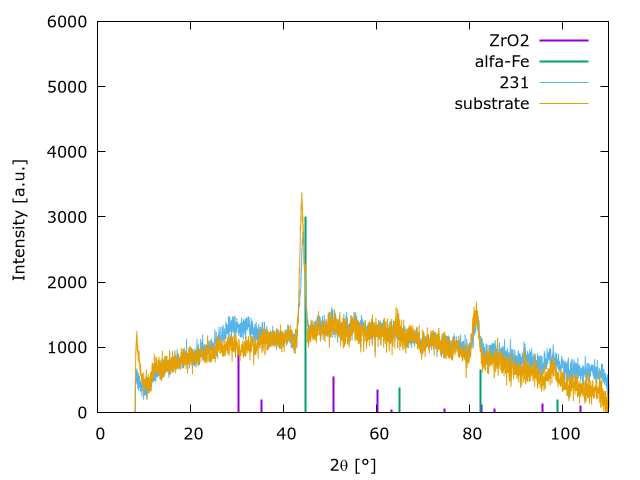
\includegraphics[width=\picwidth]{Pics/xrd.png}
	\caption{XRD spectra}
	\label{fig:xrd}
\end{figure}

%%%%%%%%%%%%%%%%%%%%%%%%%%%%%%%%%%%%%%%%%%%%%%%%%%%%%%%%%%%
%%%%%%%%%%%%%%%%%%%%%%%%%%%%%%%%%%%%%%%%%%%%%%%%%%%%%%%%%%%
\subsection{SEM}
\begin{figure}
    \centering
    \begin{subfigure}{.4\textwidth}
        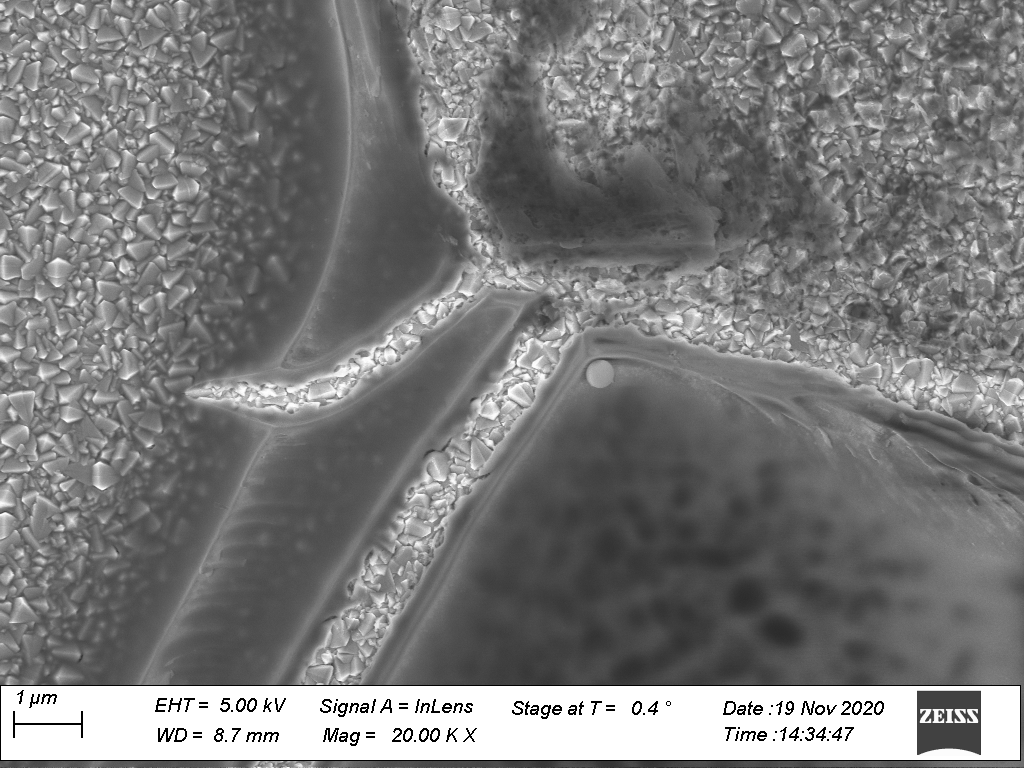
\includegraphics[width=\textwidth]{Pics/sem/071_fto_old_1x.png}
        \caption{sem1}
        \label{fig:sem1}
    \end{subfigure}
    \begin{subfigure}{.4\textwidth}
        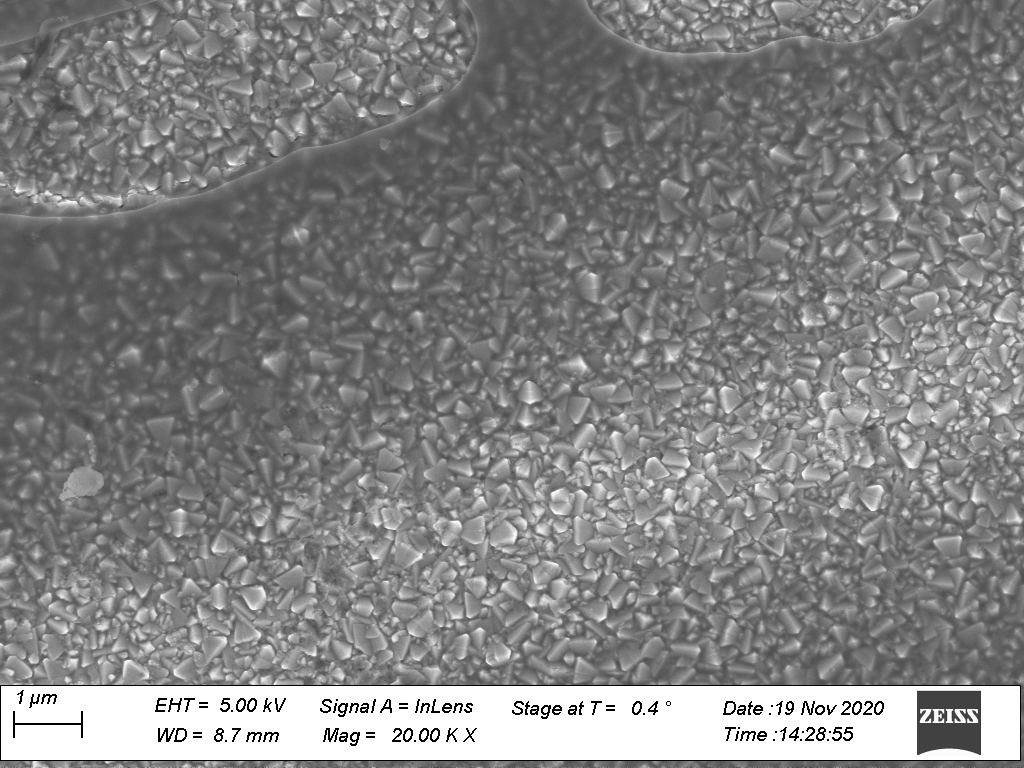
\includegraphics[width=\textwidth]{Pics/sem/071_fto_old_2x.png}
        \caption{sem2}
        \label{fig:sem2}
    \end{subfigure}
    \caption{sem}
    \label{fig:sem}
\end{figure}


%%%%%%%%%%%%%%%%%%%%%%%%%%%%%%%%%%%%%%%%%%%%%%%%%%%%%%%%%%%
%%%%%%%%%%%%%%%%%%%%%%%%%%%%%%%%%%%%%%%%%%%%%%%%%%%%%%%%%%%
\subsection{Material Scientific}
\subsubsection{First recipe} 
As already indicated in the experimental section the recipe adopted from \cite{Anwar2017} didn't produce any \td{good} results. 
The solution was milky/cloudy and didn't produce homogeneous films. 
Altering the composition, pH etc. didn't improve the resulting layers. 

The sol-gel recipe optimized by \cite{Hu2016} for \ch{Al2O3} worked splendidly for our use even after (not so) minor changes.
%An substantial improvement could be achieved by
The stability of the solution could be increased a lot by replacing the stabilizing agent (\gls{acoh}) with \gls{ipo}.
The stability was inspected visually. 
As soon as the solution showed initial cloudiness, it was declared as unstable. 
The regular solution was stable for approximately \td{24h} sealed with Parafilm. 
A solution with \gls{ipo} as stabilizing agent stayed stable for \td{72h}. 
As an increase of the \gls{zrpro} concentration decreased the \td{stable time}. 
%5F ca 100min
%4F ca 140min
%3F ca 420min (7h)
\Gls{ipo} solution allowed to even reuse high concentrated solution, which would otherwise become cloudy under 60 minutes. 
Multiple question still need to be answered: 
What causes the cloudiness (as stability increased through sealing probably \ch{H2O} from the air or \ch{O2}) and what's the mechanism? 
How does \gls{ipo} increase the stability? 
Does it do so because it "fits" better with the solvent. 
As the original solvent was 2-methoxy-ethonanol instead of \ch{buoh}. 
It was even observed that the addition of \td{some drops of} \gls{ipo} to an acetic solution can clear the solution.
5F acetic solution milky over night 5:1 dilution with \gls{ipo} and clear after one minute of stirring and stayed clear over 5 nights.
% more details on pages 68ff
No effect on the solution or the resulting layer was noticed \td{from the initial stirring}
\todo{Following stirring times (in minutes) were tested and didn't have an influence on stability of the solution: 10-10-20, 10-10-45, 30-30-180.}

%\td{instead of changing the stabilisation agent before optimisation, could change after pso, was vor und nachteile?}
after realizing the improved effectiveness of \gls{ipo} for experimentation, 
it was decided that EMMA will be executed with \gls{ipo} solution.
\begin{figure}
    \centering
    \begin{subfigure}{.3\textwidth}
        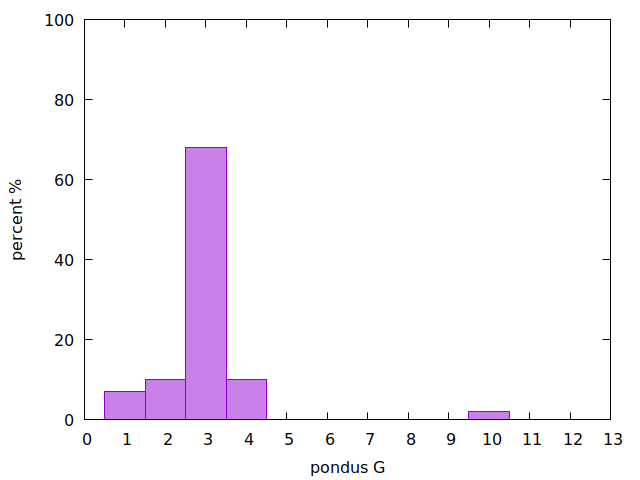
\includegraphics[width=\textwidth]{Pics/iv/iv-199-acoh.png}
        \caption{iv acoh} \label{fig:iv-acoh}
    \end{subfigure}
    \begin{subfigure}{.3\textwidth}
        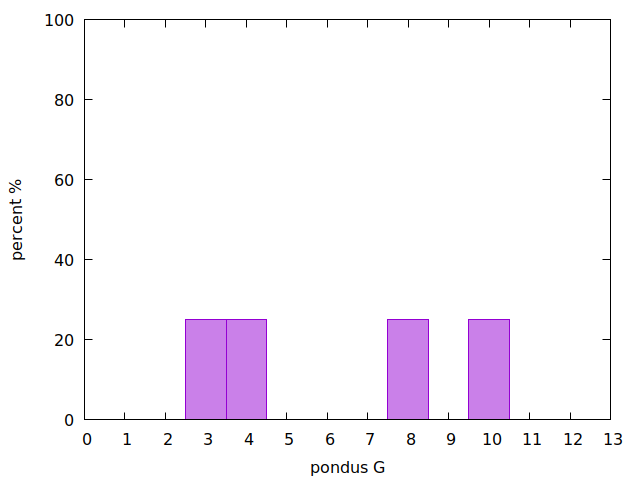
\includegraphics[width=\textwidth]{Pics/iv/iv-201-acoh-ipo.png}
        \caption{iv acoh ipo} \label{fig:iv-acoh-ipo}
    \end{subfigure}
    \begin{subfigure}{.3\textwidth}
        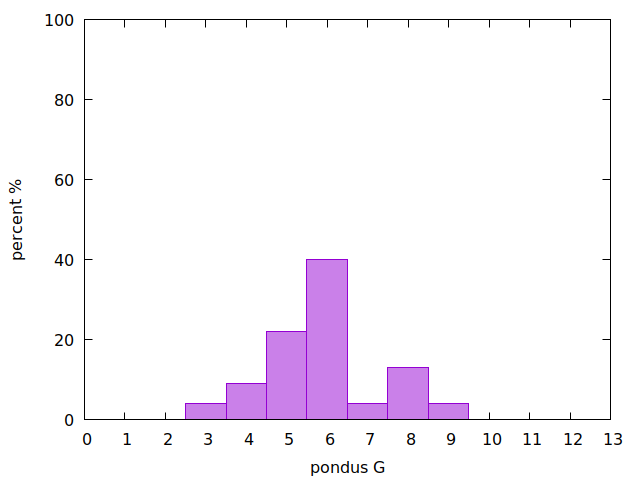
\includegraphics[width=\textwidth]{Pics/iv/iv-192-ipo.png}
        \caption{ipo} \label{fig:ipo}
    \end{subfigure}
    \caption{iv of 6x4F} \label{fig:iv}
\end{figure}

%%%%%%%%%%%%%%%%%%%%%%%%%%%%%%%%%%%%%%%%%%%%%%%%%%%%%%%%%%%
%%%%%%%%%%%%%%%%%%%%%%%%%%%%%%%%%%%%%%%%%%%%%%%%%%%%%%%%%%%
\subsection{V-I and preoptimization}
\td{varied doctor blading velocity: 10, 5, 1, 0.5, 0.2, 0.1. Slower less layer}
\td{extra PB-design with conc(2-4), layers(6-8), tcal(430-470), tvel(4-6),
vdoc(0.5-2), tdoc(40-60). low vdoc very homogenuous but actually nearly no 
deposition because miniscus is pulling liquid off the substrate.}
\td{IPO influence on "stability" p74: 600ul IPO makes clear, 4000 ul BuOH not clear with 
same base solution (1ml of 4F), added extra 400ul to BuOH sol and after 5min clear. 
of 1:5 is unacceptable Dilution }
- 21.8 (1F) from 15.02. 13:30 bis 
26.3 (1ml iPO to ca2ml of 5f) from 16.02. 16:30 bis 18.02.++
18.02 4F in 80min milky
      2F in ca 24h (stabilization AcOH)
- first recipe tried to improve to achieve more restisting layer. by pH value, surface 
tensionand solution ratios (only 10\% change because it was assumed, that the recipe is 
good and should be improved, but the recipe should be altered thoroughly.
two layers were also tried but didn't even pass the visual examination/test/inspection. 
A curst was produced. 
- At this point in time everything was doctor bladed by hand. The hight was varied (with tape).
When the switch to the erichsen was made. The height was kept constant in order to keep 
the variables to optimize ueberschuabar, but could have been even less variables.
If the movement was to slow the resluting  layer would be very inhomogenuous, thus the
velocity wasn't varied.
\td{p75 tested various vDOC (10,15,20) with TDOC (40,60,70,80) variations with only visual 
inspection of evaporation process. Ideally solution evaporate shortly after DB but not 
before} 
n-BuOH has boiling point of ca 117C\td{\cite{ncbi1butanol} look at source}
- p76, 146 (10x1F) good, 154 (3x4F) okay, 156 (3x3F) bad visualisation
- first experiments generated, but trashed because 1F solution neglected, contraints tightened
- p82 test to what extend AcOH can be replaced with iPOH
- 192 was first with IPOH
- why is IPO satbilizing? what are reasons for instability? 
\td{
acceptable layer was produced by buthanolic solution, but very unstable (short lived) how long? p41 
extra AcOH stabilzed but needed so much that dilution too large...
The stirring time was untersucht, but not much difference so shortest was used because 
short time can produces faster and the resulting solution is longer stable 
(after finishing mixing)
10 layers were tried of short stiring and gave good results? samples 130,131,134,135 (p43)
}
- \td{talk about the switch of recipe before emma: makes experiments hard/impossible to compare, but more practical and proof that it works weell} 


